\section{Validazione}

Il problema principale della SCI consiste, data una generica immagine $I$ ed un insieme $R_1, \ldots, R_m$ di \emph{reference patterns}, nello stabilire da quale sorgente è stata scattata.

Per ciascuna immagine in ingresso viene dunque estratta la PRNU stimata e comparata con le \emph{fingerprints} ottenute mediante le operazioni di clustering. Il confronto viene effettuato mediante il calcolo della PCE. Il valore della PCE ottenuto ci fornisce una stima della confidenza della relazione tra \emph{fingerprint} e PRNU dell'immagine di partenza, consentendo di scegliere la camera con la confidenza più alta.

\begin{figure}[h]
\begin{center}
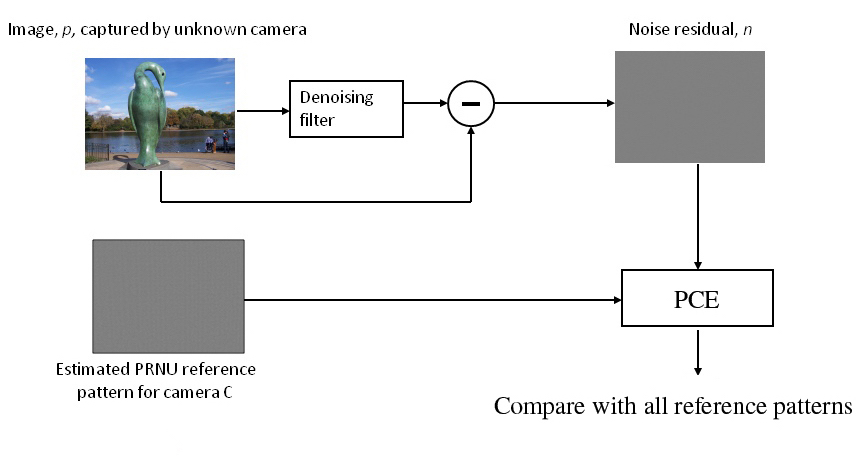
\includegraphics[width=0.45\textwidth]{images/validation.jpg}
\end{center}
  \caption{La fase di validazione di una immagine campione}
\label{fig:validation}
\end{figure}

L'operazione sopra descritta viene ripetuta su un'insieme di immagini prese dal dataset di riferimento così da poter valutare le performance del sistema implementato semplicemente andando a comparare la predizione ottenuta per ciascuna immagine con il \emph{ground-truth} posseduto.